\documentclass[landscape,a4paper]{article}
\usepackage[top=0cm, bottom=0cm, left=0.0cm, right=0.0cm]{geometry}
\usepackage{tikz}
\usetikzlibrary{patterns}
\usetikzlibrary{shapes,arrows}
\usetikzlibrary{calc}
\usetikzlibrary{decorations.pathreplacing}

\usetikzlibrary{arrows,arrows.meta}
\usepackage{amsmath}
\usepackage{amsfonts}

\usepackage{libertine}
\usepackage{libertinust1math}
\usepackage[T1]{fontenc}

\usetikzlibrary{automata,positioning}

\begin{document}
	\noindent
	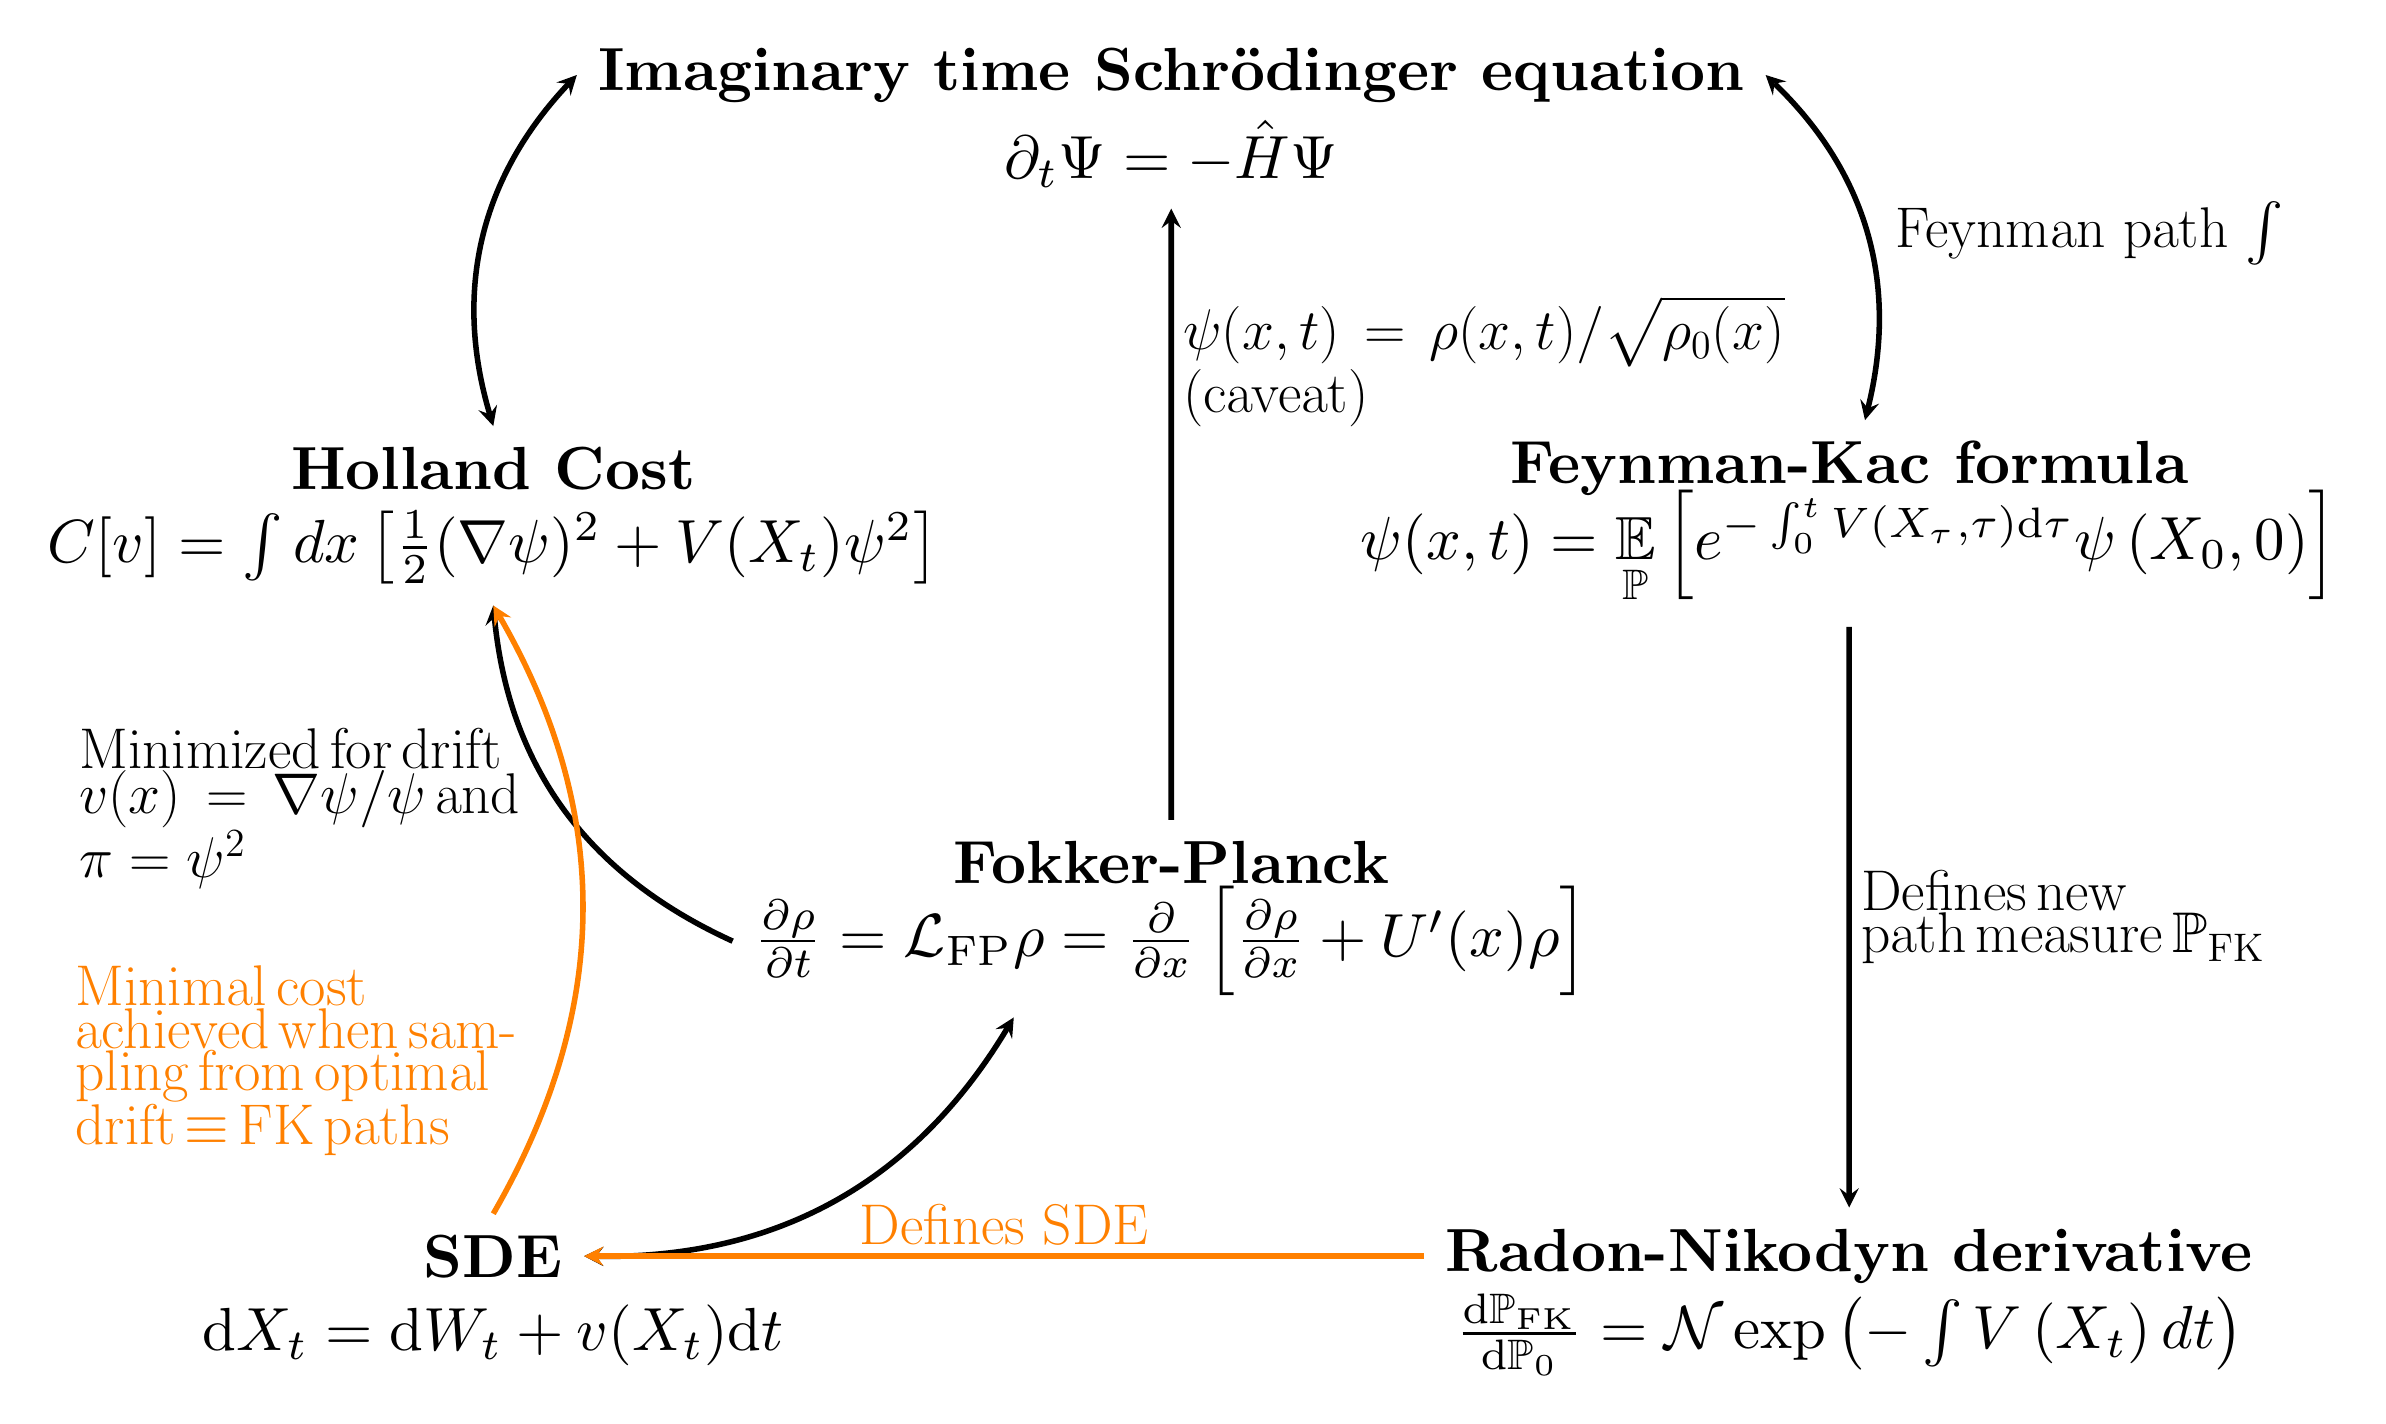
\begin{tikzpicture}[%
		>=stealth,
		node distance=3cm,
		on grid,
		auto
		]
		% (28.7cm,20cm)
		% decomposition
		%%%%%%%%%%%%%%%
		%    NODES    %
		%%%%%%%%%%%%%%%
		\node[style={rectangle}, scale=2.2] (sch) at (28.7/2, 19) {\textbf{Imaginary time Schr\" odinger equation}};
		\node[style={rectangle}, scale=2.2] (scheq) at (28.7/2, 18) {${\partial_t} \Psi = -\hat{H} \Psi$};
		
		% Control
		\node[style={rectangle}, scale=2.2] (hol) at (28.7/5, 14) {\textbf{Holland Cost}};
		\node[style={rectangle}, scale=2.2] (holeq) at (28.7/5, 13) {$C[v]=\int d x\left[\frac{1}{2}(\nabla \psi)^{2}+V(X_{t}) \psi^{2}\right]$};
		
		% FKac
		\node[style={rectangle}, scale=2.2] (fkac) at (4*28.7/5, 14) {\textbf{Feynman-Kac formula}};
		\node[style={rectangle}, scale=2.2] (fkaceq) at (4*28.7/5, 13) {$\psi(x, t)=\underset{\mathbb{P}}{\mathbb{E}}
				\left[e^{-\int_{0}^{t}  V\left(X_{\tau}, \tau \right)  \mathrm{d}\tau} \psi\left(X_{0}, 0\right)\right]$};
		
		% Fokker-Planck
		\node[style={rectangle}, scale=2.2] (fp) at (2.5*28.7/5, 9) {\textbf{Fokker-Planck}};
		\node[style={rectangle}, scale=2.2] (fpeq) at (2.5*28.7/5, 8) {$\frac{\partial \rho}{\partial t}=\mathcal{L}_{\mathrm{FP}} \rho=\frac{\partial}{\partial x}\left[\frac{\partial \rho}{\partial x}+U^{\prime}(x) \rho\right]$};
		
		% SDE
		\node[style={rectangle}, scale=2.2] (sde) at (1*28.7/5, 4) {\textbf{SDE}};
		\node[style={rectangle}, scale=2.2] (sdeeq) at (1*28.7/5, 3) {$\mathrm{d} X_{t}=\mathrm{d} W_{t}+v(X_{t}) \mathrm{d} t$};
		
		% Radon-Nikodyn
		\node[style={rectangle}, scale=2.2] (rn) at (4*28.7/5, 4) {\textbf{Radon-Nikodyn derivative}};
		\node[style={rectangle}, scale=2.2] (rneq) at (4*28.7/5, 3) {$\frac{\mathrm{d} \mathbb{P}_{\mathrm{FK}}}{\mathrm{d} \mathbb{P}_{0}}=\mathcal{N} \exp \left(-\int V\left(X_{t}\right) d t\right)$};
		
		%%%%%%%%%%%%%%%
		% CONNECTIONS %
		%%%%%%%%%%%%%%%
		
		\path[line width=2, black, <->]
		(sch.east) edge[bend left] node [right] {\huge ~Feynman path $\int$} (fkac);
		
		\path[line width=2, black, ->]
		(fkaceq.south) edge node [right, text width=6cm] {\huge Defines new \\ path measure $\mathbb{P}_{\text{FK}}$} (rn);
		
		\path[line width=2, black, <-]
		(scheq.south) edge node [near start, right, text width=8cm] {\huge $\psi(x, t)={\rho(x, t)}/{\sqrt{\rho_{0}(x)}}$ (caveat)} (fp);
		
		\path[line width=2, black, <->]
		(sde.east) edge[bend right] node [near start, right, text width=8cm] {} ($(fpeq.south)-(2, 0)$);
		
		\path[line width=2, black, <->]
		(sch.west) edge[bend right] node [midway, left, text width=5cm] {\huge} (hol.north);
		
		\path[line width=2, black, <-]
		(holeq.south) edge[bend right] node [midway, left, text width=6cm] {\huge Minimized for drift $v(x) = \nabla \psi / \psi$ and $\pi=\psi^{2}$} (fpeq.west);
		
		% Most important last connection
		\path[line width=2, orange, ->]
		(rn.west) edge node [midway, above] {\huge Defines SDE} (sde.east);
		
		\path[line width=2, orange, <-]
		(holeq.south) edge[bend left] node [near end, left, text width=6cm] {\huge Minimal cost achieved when sampling from optimal drift $\equiv$ FK paths} (sde.north);
		
	\end{tikzpicture}%
\end{document}